%%%%%%%%%%%%%%%%%%%%%%%%%%%%%%%%%%%%%%%%%%%%%%%%%%%%%%%%%%%
%
%--------------CAPÍTULO 4 - MATERIAIS E MÉTODOS-------------
%
%
\chapter{Materiais e Métodos}
\label{cap:materiais-metodos}

Este capítulo descreve como a solução foi construída e avaliada. A Seção~\ref{sec:visao-geral-metodo} apresenta as etapas do trabalho e a ordem em que foram executadas. A Seção~\ref{sec:aquisicao} descreve o ambiente experimental e a aquisição dos vídeos, e a Seção~\ref{sec:prova-conceito} descreve o teste preliminar com um detector pré-treinado. A Seção~\ref{sec:base-deteccao} trata da construção e da caracterização da base de imagens usada pelos detectores. A Seção~\ref{sec:protocolo-validacao} detalha o protocolo de validação cruzada por blocos temporais. As Seções~\ref{sec:especialistas} e~\ref{sec:baseline} descrevem o treinamento dos detectores especialistas e do baseline monolítico, e as Seções~\ref{sec:roteamento} e~\ref{sec:metodo-oclusao}, o treinamento e a análise de interpretabilidade da rede de roteamento. A Seção~\ref{sec:arquitetura-moe} apresenta a arquitetura integrada e o \textit{pipeline} de inferência. A Seção~\ref{sec:avaliacao-videos} descreve a avaliação em vídeos de teste independentes, e a Seção~\ref{sec:ambiente-computacional}, o ambiente computacional usado nos experimentos.

\section{Visão Geral da Metodologia}
\label{sec:visao-geral-metodo}

O trabalho seguiu uma sequência de etapas em que cada uma dependeu da anterior. Primeiro, um detector YOLOv8 pré-treinado no COCO foi aplicado diretamente às imagens da baia, sem nenhum ajuste, para verificar se um modelo de propósito geral bastaria. Como não bastou, foi construída uma base de imagens rotuladas a partir dos vídeos do projeto, organizada pelos quatro cenários de captura: Frontal Dia, Frontal Noite, Superior Dia e Superior Noite.

As primeiras rodadas de treinamento usaram particionamento aleatório das imagens entre treino e validação e produziram métricas muito próximas do máximo. Como as imagens são quadros de vídeo, essa proximidade levantou a suspeita de vazamento de dados entre quadros vizinhos (Seção~\ref{sec:validacao-cruzada-vazamento}). Os resultados dessas rodadas foram descartados, e todos os modelos reportados neste trabalho foram treinados e avaliados sob o protocolo de validação cruzada por blocos temporais descrito na Seção~\ref{sec:protocolo-validacao}.

Sob esse protocolo, foram treinados quatro detectores especialistas, um por cenário, e um detector único sobre a união dos quatro cenários, que serve de baseline. Em paralelo, uma rede de classificação foi treinada para reconhecer o cenário de captura a partir de uma imagem e teve suas decisões analisadas por oclusão. Por fim, a rede de roteamento e os especialistas foram integrados em um \textit{pipeline} de inferência sobre vídeo, e as duas abordagens (MoE e baseline) foram comparadas em quatro vídeos que não fizeram parte do treinamento.

\section{Ambiente Experimental e Aquisição dos Vídeos}
\label{sec:aquisicao}

Os dados foram coletados em uma baia experimental da UFSJ que abriga um rebanho de oito cabras da raça \textit{Saanen}. Os mesmos oito animais permaneceram na baia durante todo o período de aquisição e aparecem em todos os cenários de captura. A baia é monitorada por quatro câmeras fixas, identificadas como Cam01, Cam02, Cam03 e Cam04, instaladas em duas perspectivas: frontal, com a câmera voltada para a frente da baia, e superior (zenital), com a câmera posicionada acima dos animais. As câmeras Cam01 e Cam03 registram a perspectiva frontal, e as câmeras Cam02 e Cam04, a superior.

Durante o dia, as imagens são coloridas e iluminadas por luz natural. À noite, as câmeras passam a operar no espectro infravermelho e produzem imagens monocromáticas. Da combinação entre as duas perspectivas e as duas condições de iluminação resultam os quatro cenários de captura que organizam todo o trabalho.

Os vídeos foram gravados na resolução nativa de 1280$\times$960 pixels, a 8 quadros por segundo (FPS). Ao todo, foram usadas 36 sessões de gravação, distribuídas em sete dias de aquisição entre 25 de abril e 3 de maio de 2025 e realizadas em horários variados, tanto de dia quanto de madrugada. Cada sessão é um trecho contínuo de vídeo de uma única câmera, e o número de quadros aproveitados por sessão variou de 40 a 1.670. Os arquivos seguem um padrão de nome que registra a câmera, a data e o horário de início da gravação (por exemplo, \texttt{Cam03\_2025\_04\_25\_16\_17\_49\_capril}), e esse padrão foi usado mais tarde para agrupar as imagens por sessão (Seção~\ref{sec:protocolo-validacao}).

\section{Prova de Conceito com Detector Pré-Treinado}
\label{sec:prova-conceito}

Antes de construir uma base própria, verificou-se se um detector de propósito geral seria suficiente. Para isso, o YOLOv8m com pesos pré-treinados no COCO \cite{jocher2023yolov8, journals/corr/LinMBHPRDZ14} foi aplicado diretamente a quadros extraídos dos vídeos, sem nenhum treinamento adicional. Como o COCO não tem uma classe para caprinos, as detecções foram filtradas pela classe morfologicamente mais próxima, \textit{sheep} (ovelha). O teste incluiu imagens diurnas e noturnas e as duas perspectivas. O critério de avaliação foi qualitativo: verificar se o modelo encontrava os oito animais da baia e com que confiança. Os resultados desse teste, que motivaram a construção da base própria, estão no Capítulo~5.

\section{Construção da Base de Imagens para Detecção}
\label{sec:base-deteccao}

\subsection{Extração dos Quadros e Rotulação}
\label{subsec:rotulacao}

Os quadros de cada sessão foram extraídos dos vídeos e mantidos na ordem em que foram gravados. Nas sessões usadas neste trabalho, os quadros foram aproveitados sem subamostragem adicional além da taxa de 8 FPS da câmera, o que preserva a sequência temporal de cada gravação e permite reconstruí-la a partir do índice do quadro, registrado no nome do arquivo. \todo{Rever: a marcação de hora gravada nas imagens mostra que ao menos parte das sessões foi subamostrada. A sessão \texttt{Cam03\_2025\_04\_26\_18\_17\_10} tem 140 quadros entre 18h17min10s e 19h16min40s (cerca de um quadro a cada 26 s), e as três sessões da Cam04 de 26/04 têm 125--150 quadros em cerca de uma hora cada. Nessas sessões, a zona de purga de 15 quadros corresponde a uns 6 minutos, e não a 2 segundos. O nome dos quadros das quatro sessões curtas da Cam02 em Superior Dia (\texttt{\ldots\_random\_N}) sugere amostragem aleatória, caso em que o índice não garante a ordem temporal.}

A rotulação foi manual e seguiu a definição de uma única classe, \texttt{goat}. Cada animal visível na baia principal foi delimitado por uma caixa ajustada ao seu contorno, de modo a deixar o mínimo de fundo dentro da caixa. Esses critérios foram estabelecidos em um guia de rotulação elaborado nas primeiras fases do projeto, quando a anotação era feita por voluntários da UFJF e da UFSJ na ferramenta \textit{Makesense.ai}. A base final foi rotulada por alunos da UFSJ com o auxílio do EasyLabel\footnote{Disponível em: \url{https://github.com/Gabriel0Bernardini/EasyLabel}.}, uma ferramenta desenvolvida por eles para padronizar a anotação e organizar os arquivos no formato exigido pelo YOLO. \todo{Confirmar com a equipe da UFSJ se os critérios do guia original (apenas animais da baia principal, caixas justas) foram mantidos na rotulação com o EasyLabel.}

No formato YOLO, cada imagem tem um arquivo de texto com o mesmo nome, e cada linha desse arquivo descreve uma caixa:
\begin{equation}
    c \quad x_c \quad y_c \quad w \quad h,
    \label{eq:formato-yolo}
\end{equation}
em que $c$ é o índice da classe (sempre 0, correspondente a \texttt{goat}), $(x_c, y_c)$ são as coordenadas do centro da caixa, e $w$ e $h$ são sua largura e altura. As quatro coordenadas são normalizadas pelas dimensões da imagem e ficam, portanto, no intervalo $[0, 1]$, o que as torna independentes da resolução em que a imagem é processada.

\subsection{Organização e Verificação da Base}
\label{subsec:organizacao-base}

As imagens foram separadas em quatro pastas, uma por cenário de captura, cada uma com subpastas de imagens e de rótulos. Parte das imagens passou pela plataforma Roboflow antes de chegar à base final, e essas imagens receberam nomes no padrão de exportação da plataforma, com um sufixo de identificação. As imagens incorporadas na última expansão da base foram extraídas diretamente dos vídeos e mantêm o nome original da sessão seguido do índice do quadro. Os dois padrões preservam a sessão de origem e a posição do quadro na gravação.

Na última expansão, a base passou de 5.204 para 8.604 imagens. Durante essa expansão, verificou-se que parte das imagens novas havia sido depositada em subpastas aninhadas e com um padrão de nome que o \textit{script} de particionamento não reconhecia, de modo que essas imagens ficariam fora do treinamento sem nenhum aviso. O \textit{script} foi corrigido para buscar imagens de forma recursiva e para reconhecer o novo padrão de nome, e a estrutura de pastas foi reorganizada sem perda de arquivos. Também foi confirmado que a biblioteca de treinamento associava corretamente cada imagem ao seu arquivo de rótulos após a reorganização.

Antes do treinamento, a base passou por três verificações automáticas: nenhum arquivo de rótulos estava vazio, todas as imagens tinham um arquivo de rótulos correspondente (e vice-versa), e todas as caixas pertenciam à classe 0. Todas as 8.604 imagens seguiam um dos padrões de nome reconhecidos, de modo que nenhuma foi descartada por falta de informação sobre sua posição temporal.

\subsection{Caracterização da Base}
\label{subsec:caracterizacao-base}

A Tabela~\ref{tab:dataset-deteccao} resume a base de detecção por cenário. Ao todo, são 8.604 imagens e 68.832 caixas delimitadoras, provenientes das 36 sessões de gravação. Os cenários têm tamanhos parecidos, entre 2.001 e 2.549 imagens, o que evita que algum especialista seja treinado com muito menos dados que os demais.

\begin{table}[htb]
\centering
\caption{Caracterização da base de detecção por cenário de captura.}
\label{tab:dataset-deteccao}
\begin{tabular}{lcrrrr}
\hline
\textbf{Cenário} & \textbf{Câmeras} & \textbf{Sessões} & \textbf{Imagens} & \textbf{Caixas} & \textbf{Caixas/imagem} \\
\hline
Frontal Dia & Cam01, Cam03 & 8 & 2.022 & 16.185 & 8,00 \\
Frontal Noite & Cam03 & 13 & 2.001 & 16.009 & 8,00 \\
Superior Dia & Cam02, Cam04 & 6 & 2.549 & 20.384 & 8,00 \\
Superior Noite & Cam02, Cam04 & 9 & 2.032 & 16.254 & 8,00 \\
\hline
\textbf{Total} & Cam01--Cam04 & \textbf{36} & \textbf{8.604} & \textbf{68.832} & 8,00 \\
\hline
\end{tabular}

\vspace{0.2cm}
Fonte: Elaborada pelo autor.
\end{table}

Nos quatro cenários, a média é de oito caixas por imagem, o que corresponde ao rebanho completo. Das 8.604 imagens, 8.555 (99,4\%) têm exatamente oito caixas. As 49 restantes têm entre seis e nove caixas, com exceção de uma imagem de Superior Dia com 13 caixas, número incompatível com o rebanho e que indica erro de anotação. O número de sessões também varia entre os cenários, de 6 em Superior Dia a 13 em Frontal Noite. Esse número importa para a avaliação, porque um cenário com poucas sessões oferece menos variedade de dias e horários, e os blocos de validação desse cenário tendem a se parecer mais com os de treino.

\section{Protocolo de Validação Cruzada por Blocos Temporais}
\label{sec:protocolo-validacao}

\subsection{Motivação}
\label{subsec:motivacao-protocolo}

A 8 FPS, a posição e a postura dos animais mudam pouco de um quadro para o seguinte, e quadros vizinhos de uma mesma sessão são quase idênticos. Em uma validação cruzada \textit{K-Fold} convencional, cada imagem é sorteada de forma independente para um dos \textit{folds}, e a chance de um quadro de validação ter um vizinho imediato no treino é muito alta. O modelo seria, então, avaliado sobre imagens praticamente iguais às que viu durante o ajuste dos pesos, e as métricas superestimariam sua capacidade de generalização \cite{kaufman2012leakage, roberts2017crossvalidation}. Foi o que se observou nas primeiras rodadas de experimentos deste trabalho, motivo pelo qual o protocolo descrito a seguir foi adotado em todos os treinamentos dos detectores.

\subsection{Particionamento em Blocos Temporais Contíguos}
\label{subsec:blocos-temporais}

O protocolo divide cada sessão em blocos contíguos de tempo, em vez de sortear quadros individuais. O procedimento tem quatro passos.

Primeiro, cada imagem é associada à sua sessão de origem e ao índice do quadro dentro da sessão, ambos extraídos do nome do arquivo por expressões regulares que cobrem os padrões de nome existentes na base. Uma imagem cujo nome não segue nenhum desses padrões seria excluída do particionamento, pois não haveria como saber sua posição na sequência; na base final, nenhuma imagem precisou ser excluída.

Segundo, as imagens de cada sessão são ordenadas pelo índice do quadro. Seja $s$ uma sessão com $n_s$ imagens ordenadas, indexadas por $i = 0, \ldots, n_s - 1$. Com $K = 5$ \textit{folds}, a sessão é dividida em cinco blocos consecutivos de tamanho aproximadamente igual, e a imagem de posição $i$ é atribuída ao bloco
\begin{equation}
    b_s(i) = \min\left( \left\lfloor \frac{i}{n_s / K} \right\rfloor ,\; K - 1 \right).
    \label{eq:bloco-temporal}
\end{equation}

Terceiro, no \textit{fold} $f \in \{1, \ldots, K\}$, as imagens do bloco $f$ de cada sessão formam o conjunto de validação daquela sessão, e as dos demais blocos são candidatas ao treino. Como esse procedimento é aplicado a todas as sessões, cada \textit{fold} reserva para validação cerca de 20\% da linha do tempo de cada sessão, e cada sessão contribui tanto para o treino quanto para a validação de todos os \textit{folds}. Ao longo dos cinco \textit{folds}, cada imagem aparece exatamente uma vez na validação.

Quarto, aplica-se uma zona de exclusão (\textit{purge buffer}) em torno do bloco de validação. Mesmo com blocos contíguos, os quadros imediatamente anteriores e posteriores ao bloco de validação são quase idênticos aos quadros da borda desse bloco. Para reduzir essa dependência, as $p = 15$ imagens imediatamente anteriores e as $p$ imediatamente posteriores ao bloco de validação são removidas do treino daquele \textit{fold}. Sendo $[a_f, e_f)$ o intervalo de posições do bloco de validação $f$ em uma sessão, o conjunto de treino dessa sessão no \textit{fold} $f$ é
\begin{equation}
    \mathcal{T}_f = \left\{ i \;:\; b_s(i) \neq f \;\text{ e }\; i \notin [\, a_f - p,\; e_f + p \,) \right\},
    \label{eq:purge}
\end{equation}
e as imagens da zona de exclusão não entram nem no treino nem na validação desse \textit{fold}. Quando os quadros de uma sessão são consecutivos, 15 imagens correspondem a cerca de 1,9 segundo de vídeo de cada lado do bloco. Essa estratégia de descartar amostras na fronteira entre treino e teste é usada em validação de modelos sobre séries temporais, em que é conhecida como \textit{purging} \cite{lopezdeprado2018advances}. O Algoritmo~\ref{alg:kfold-temporal} resume o procedimento.

\begin{algorithm}[htb]
\caption{Particionamento \textit{K-Fold} por blocos temporais com zona de exclusão.}
\label{alg:kfold-temporal}
\SetKwInput{KwIn}{Entrada}\SetKwInput{KwOut}{Saída}
\SetKwFor{ForEach}{para cada}{faça}{fim}\SetKwFor{For}{para}{faça}{fim}
\SetKwIF{If}{ElseIf}{Else}{se}{então}{senão se}{senão}{fim}\SetKw{KwTo}{até}
\KwIn{conjunto de imagens $\mathcal{D}$; número de \textit{folds} $K$; tamanho da zona de exclusão $p$}
\KwOut{conjuntos de treino $\mathcal{T}_f$ e de validação $\mathcal{V}_f$, para $f = 1, \ldots, K$}
Agrupar as imagens de $\mathcal{D}$ por sessão, a partir do nome do arquivo\;
\ForEach{sessão $s$}{
    Ordenar as imagens de $s$ pelo índice do quadro\;
    Atribuir cada posição $i$ ao bloco $b_s(i)$ (Equação~\ref{eq:bloco-temporal})\;
    \For{$f \leftarrow 1$ \KwTo $K$}{
        $[a_f, e_f) \leftarrow$ intervalo de posições do bloco $f$\;
        \ForEach{posição $i$ em $s$}{
            \uIf{$b_s(i) = f$}{adicionar a imagem $i$ a $\mathcal{V}_f$\;}
            \uElseIf{$a_f - p \leq i < e_f + p$}{descartar a imagem $i$ no \textit{fold} $f$\;}
            \Else{adicionar a imagem $i$ a $\mathcal{T}_f$\;}
        }
    }
}
Verificar que $\mathcal{T}_f \cap \mathcal{V}_f = \emptyset$ para todo $f$\;
\end{algorithm}

O particionamento foi feito separadamente para cada um dos quatro cenários, gerando os \textit{folds} dos especialistas, e mais uma vez sobre a base unificada, gerando os \textit{folds} do baseline. Como a divisão é feita sessão a sessão, e cada sessão pertence a um único cenário, o bloco de validação de uma sessão é o mesmo nos dois casos: o \textit{fold} $f$ do baseline contém exatamente a união das imagens de validação do \textit{fold} $f$ dos quatro especialistas. Isso torna a comparação entre as duas abordagens justa, pois ambas são avaliadas sobre os mesmos trechos de vídeo em cada \textit{fold}.

\subsection{Auditoria do Particionamento}
\label{subsec:auditoria}

Para cada \textit{fold}, o \textit{script} de particionamento verificou que nenhum arquivo aparece ao mesmo tempo no treino e na validação, e registrou em um relatório o número de sessões, o número de imagens excluídas e o tamanho de cada conjunto. A Tabela~\ref{tab:auditoria-folds} apresenta esses números. A zona de exclusão removeu 4.234 amostras somando os cinco \textit{folds} da base unificada, o mesmo total obtido somando as remoções dos quatro especialistas (960, 1.544, 664 e 1.066). O cenário Frontal Noite é o que perde mais imagens para a zona de exclusão porque tem mais sessões (13), e cada sessão pode perder até 30 imagens por \textit{fold}, 15 em cada borda do bloco de validação.

\begin{table}[htb]
\centering
\caption{Tamanho dos conjuntos de treino e de validação (treino/validação) em cada \textit{fold}, após a aplicação da zona de exclusão.}
\label{tab:auditoria-folds}
\footnotesize
\setlength{\tabcolsep}{4pt}
\begin{tabular}{lrrrrrr}
\hline
\textbf{Modelo} & \textbf{Fold 1} & \textbf{Fold 2} & \textbf{Fold 3} & \textbf{Fold 4} & \textbf{Fold 5} & \textbf{Excluídas} \\
\hline
Frontal Dia & 1.496/406 & 1.378/404 & 1.378/404 & 1.378/404 & 1.498/404 & 960 \\
Frontal Noite & 1.405/401 & 1.219/400 & 1.211/400 & 1.219/400 & 1.406/400 & 1.544 \\
Superior Dia & 1.949/510 & 1.887/510 & 1.859/510 & 1.887/510 & 1.950/509 & 664 \\
Superior Noite & 1.490/407 & 1.363/406 & 1.355/407 & 1.363/406 & 1.491/406 & 1.066 \\
\hline
Baseline (unificado) & 6.340/1.724 & 5.847/1.720 & 5.803/1.721 & 5.847/1.720 & 6.345/1.719 & 4.234 \\
\hline
\end{tabular}

\vspace{0.2cm}
\normalsize
Fonte: Elaborada pelo autor. A coluna ``Excluídas'' soma as imagens removidas pela zona de exclusão nos cinco \textit{folds}.
\end{table}

Os \textit{folds} 1 e 5 têm conjuntos de treino maiores que os demais. Nesses \textit{folds}, o bloco de validação fica no início ou no fim de cada sessão e, por isso, só tem uma borda vizinha a imagens de treino, de modo que a zona de exclusão remove metade das imagens que remove nos \textit{folds} intermediários.

\subsection{Limitações do Protocolo}
\label{subsec:limitacoes-protocolo}

O protocolo reduz o vazamento entre quadros vizinhos, mas não separa sessões inteiras. Como todas as sessões participam do treino e da validação de todos os \textit{folds}, o modelo é validado sobre um trecho de uma gravação cujos outros trechos ele viu no treino, com o mesmo fundo, a mesma câmera, os mesmos animais e iluminação semelhante. Nos cenários com menos sessões, como Superior Dia, essa semelhança tende a ser maior. Uma avaliação mais rigorosa exigiria reservar sessões ou dias inteiros para validação, por exemplo com um \textit{Group K-Fold} por sessão. Essa alternativa não foi adotada neste trabalho e é apontada como trabalho futuro; com apenas seis sessões no cenário Superior Dia, ela também exigiria cuidado para que os \textit{folds} tivessem tamanhos comparáveis. Para compensar essa limitação, os modelos finais também foram avaliados em vídeos de teste que não pertencem a nenhuma sessão do treinamento (Seção~\ref{sec:avaliacao-videos}).

\section{Treinamento dos Detectores Especialistas}
\label{sec:especialistas}

Cada especialista é um YOLOv8 na variante \textit{medium} (YOLOv8m) \cite{jocher2023yolov8}, inicializado com os pesos pré-treinados no COCO e ajustado apenas com as imagens do seu cenário. A variante \textit{medium} foi escolhida como compromisso entre precisão e custo computacional, considerando que o trabalho previa 25 treinamentos completos (5 \textit{folds} para cada um dos quatro especialistas e para o baseline). O detector tem uma única classe de saída, \texttt{goat}.

Os hiperparâmetros usados estão na Tabela~\ref{tab:hiperparametros-yolo}. As imagens são redimensionadas para 640$\times$640 pixels na entrada da rede. O tamanho do lote foi definido pelo mecanismo AutoBatch da biblioteca Ultralytics (parâmetro \texttt{batch=-1}), que estima o maior lote que cabe na memória da GPU. O treinamento foi limitado a 300 épocas, com parada antecipada quando a métrica de validação não melhora por 30 épocas consecutivas (\texttt{patience=30}). A biblioteca acompanha, para essa parada e para a escolha dos pesos salvos, uma métrica de aptidão (\textit{fitness}) que combina mAP50 e mAP50-95, com peso maior para a segunda. O otimizador, a taxa de aprendizado e o aumento de dados (como composição em mosaico, variações de matiz, saturação e brilho, espelhamento horizontal, translação e escala) foram mantidos nos valores padrão da biblioteca, iguais para todos os modelos.

\begin{table}[htb]
\centering
\caption{Hiperparâmetros de treinamento dos detectores YOLOv8m (especialistas e baseline).}
\label{tab:hiperparametros-yolo}
\begin{tabular}{ll}
\hline
\textbf{Parâmetro} & \textbf{Valor} \\
\hline
Arquitetura & YOLOv8m (pré-treinado no COCO) \\
Classes & 1 (\texttt{goat}) \\
Resolução de entrada & 640$\times$640 pixels \\
Épocas (máximo) & 300 \\
Parada antecipada & 30 épocas sem melhora (\texttt{patience=30}) \\
Tamanho do lote & automático (\texttt{batch=-1}, AutoBatch) \\
\textit{Cache} de imagens & memória RAM (\texttt{cache='ram'}) \\
Processos de leitura de dados & 8 (\texttt{workers=8}) \\
Otimizador e aumento de dados & padrões da biblioteca Ultralytics \\
Validação & 5 \textit{folds} por blocos temporais, $p = 15$ \\
\hline
\end{tabular}

\vspace{0.2cm}
Fonte: Elaborada pelo autor.
\end{table}

Os quatro especialistas foram treinados nos cinco \textit{folds} de seus cenários, em um total de 20 treinamentos. Cada treinamento partiu novamente dos pesos do COCO, de modo que nenhum \textit{fold} herdou pesos ajustados em outro. Os treinamentos foram executados em sequência, um de cada vez, porque a execução de dois treinamentos simultâneos na única GPU disponível esgotava sua memória. Como a base estava armazenada em discos rígidos mecânicos, a leitura das imagens era o gargalo do treinamento; por isso, as imagens decodificadas foram mantidas em memória RAM depois da primeira época, e o número de processos de leitura foi elevado para 8.

Ao final de cada treinamento, a biblioteca registra as métricas de validação de todas as épocas: precisão, revocação, mAP50 e mAP50-95, definidas na Seção~\ref{sec:metricas-avaliacao}. O F1-\textit{score} foi calculado a partir da precisão e da revocação (Equação~\ref{eq:f1}). Para cada \textit{fold}, foram extraídas as métricas da época com maior mAP50; para cada especialista, foi escolhido o \textit{fold} com maior mAP50 entre os cinco, e os pesos salvos nesse \textit{fold} foram os usados na arquitetura integrada (Seção~\ref{sec:arquitetura-moe}).

\section{Treinamento do Baseline Monolítico}
\label{sec:baseline}

Para avaliar se a especialização traz algum ganho, foi treinado um detector único sobre a união das 8.604 imagens dos quatro cenários, sem roteamento e sem nenhuma informação sobre o cenário de cada imagem. Esse baseline monolítico representa a alternativa mais simples à arquitetura proposta: um só detector que precisa aprender, nos mesmos parâmetros, todas as combinações de perspectiva e iluminação.

Para que a comparação isole o efeito da arquitetura, o baseline seguiu exatamente as mesmas condições dos especialistas: o mesmo modelo de partida (YOLOv8m pré-treinado no COCO), os mesmos hiperparâmetros (Tabela~\ref{tab:hiperparametros-yolo}) e o mesmo protocolo de validação, com $K = 5$ e zona de exclusão de 15 imagens. Como explicado na Seção~\ref{subsec:blocos-temporais}, a validação de cada \textit{fold} do baseline é composta pelas mesmas imagens que formam a validação desse \textit{fold} nos quatro especialistas.

Os cinco \textit{folds} foram treinados em sequência, cada um a partir dos pesos do COCO. Todos foram interrompidos pela parada antecipada antes do limite de 300 épocas, após 224, 126, 106, 139 e 145 épocas, respectivamente. A rodada completa levou cerca de 15 horas na GPU usada nos experimentos, com o \textit{fold} mais longo próximo de 4 horas e 40 minutos. As métricas e a escolha do melhor \textit{fold} seguiram o mesmo critério dos especialistas, e os pesos do \textit{fold} escolhido foram os usados na avaliação em vídeo (Seção~\ref{sec:avaliacao-videos}).

\section{Rede de Roteamento}
\label{sec:roteamento}

\subsection{Base de Imagens de Cenário}
\label{subsec:base-roteamento}

A rede de roteamento resolve uma tarefa de classificação de imagens com quatro classes, uma por cenário: \texttt{class\_1} (Frontal Dia), \texttt{class\_2} (Frontal Noite), \texttt{class\_3} (Superior Dia) e \texttt{class\_4} (Superior Noite). Como a tarefa é reconhecer o cenário, e não localizar animais, essa rede não precisa de caixas delimitadoras: basta saber de que cenário vem cada imagem, informação dada pela pasta de vídeos de onde a imagem foi extraída.

A base foi montada a partir de vídeos separados por cenário. De cada cenário, foram extraídos quadros em intervalos regulares ao longo dos vídeos, com um limite de 1.000 quadros por cenário; quando o cenário tinha menos quadros disponíveis que esse limite, todos foram usados. Os quadros de cada cenário foram então divididos aleatoriamente na proporção 80/20 entre treino e validação, com semente fixa, o que mantém a proporção entre as classes nos dois conjuntos. O resultado foram 1.360 imagens, 1.088 para treino e 272 para validação, distribuídas como mostra a Tabela~\ref{tab:dataset-roteamento}.

Os vídeos de origem são 17 trechos curtos, de 80 quadros (10 segundos) cada, todos gravados em 25 de abril de 2025 por apenas duas câmeras: Cam01, de perspectiva frontal (sete vídeos diurnos e um noturno), e Cam02, de perspectiva superior (seis vídeos diurnos e três noturnos). Como nenhum cenário chegou ao limite de 1.000 quadros, todos os quadros foram usados, e o número de imagens de cada classe é 80 vezes o número de vídeos do cenário. Nenhum desses vídeos pertence às sessões da base de detecção, já que as sessões das câmeras Cam01 e Cam02 na base de detecção são todas de 28 de abril. Em compensação, a rede de roteamento não viu, no treinamento, nenhuma imagem das câmeras Cam03 e Cam04, que fornecem a maior parte da base de detecção e todos os vídeos de teste (Seção~\ref{subsec:videos-teste}). A classe Frontal Noite, em particular, vem de um único vídeo de 10 segundos da Cam01.

\begin{table}[htb]
\centering
\caption{Distribuição das imagens da base da rede de roteamento por cenário.}
\label{tab:dataset-roteamento}
\begin{tabular}{llrrr}
\hline
\textbf{Classe} & \textbf{Cenário} & \textbf{Treino} & \textbf{Validação} & \textbf{Total} \\
\hline
\texttt{class\_1} & Frontal Dia & 448 & 112 & 560 \\
\texttt{class\_2} & Frontal Noite & 64 & 16 & 80 \\
\texttt{class\_3} & Superior Dia & 384 & 96 & 480 \\
\texttt{class\_4} & Superior Noite & 192 & 48 & 240 \\
\hline
\textbf{Total} & & \textbf{1.088} & \textbf{272} & \textbf{1.360} \\
\hline
\end{tabular}

\vspace{0.2cm}
Fonte: Elaborada pelo autor.
\end{table}

A base é estratificada, mas não é balanceada: a classe Frontal Dia tem sete vezes mais imagens que a classe Frontal Noite. Além disso, ao contrário da base de detecção, a divisão entre treino e validação foi aleatória por quadro, de modo que quadros próximos de um mesmo vídeo podem estar nos dois conjuntos. As métricas de validação dessa rede devem, portanto, ser lidas com a mesma ressalva discutida na Seção~\ref{subsec:motivacao-protocolo}; o comportamento da rede em vídeos não vistos é verificado na avaliação da Seção~\ref{sec:avaliacao-videos}.

\subsection{Arquitetura e Treinamento}
\label{subsec:treino-roteamento}

A rede de roteamento é uma EfficientNet-B0 \cite{tan2019efficientnet}, na implementação da biblioteca \textit{torchvision}, inicializada com pesos pré-treinados no ImageNet. A última camada da cabeça de classificação foi substituída por uma camada linear com quatro saídas, uma por cenário. Todos os pesos da rede, e não apenas os da nova camada, foram ajustados durante o treinamento.

As imagens de treino passaram por um recorte aleatório com redimensionamento para 224$\times$224 pixels e por espelhamento horizontal aleatório. As imagens de validação foram redimensionadas para 256 pixels no menor lado e recortadas no centro em 224$\times$224 pixels. Nos dois casos, os valores dos pixels foram normalizados com a média e o desvio-padrão por canal do ImageNet, os mesmos usados no pré-treinamento da rede.

O treinamento usou o otimizador Adam \cite{kingma2015adam} com taxa de aprendizado de 0,001, a entropia cruzada como função de perda e lotes de 32 imagens, com limite de 50 épocas. A parada antecipada monitorou a perda de validação: o treinamento era interrompido quando essa perda não diminuía pelo menos 0,001 em relação ao melhor valor por 7 épocas seguidas. Ao longo do treinamento, foram guardados os pesos da época com maior acurácia de validação, e esses foram os pesos usados na arquitetura final. Ao final, a rede foi avaliada no conjunto de validação por precisão, revocação e F1-\textit{score} por classe e por uma matriz de confusão. A Tabela~\ref{tab:hiperparametros-roteamento} resume a configuração.

\begin{table}[htb]
\centering
\caption{Configuração de treinamento da rede de roteamento.}
\label{tab:hiperparametros-roteamento}
\begin{tabular}{ll}
\hline
\textbf{Parâmetro} & \textbf{Valor} \\
\hline
Arquitetura & EfficientNet-B0 (pré-treinada no ImageNet) \\
Camada de saída & \texttt{Linear(1280, 4)} \\
Resolução de entrada & 224$\times$224 pixels \\
Aumento de dados (treino) & recorte aleatório e espelhamento horizontal \\
Normalização & média e desvio-padrão do ImageNet \\
Otimizador & Adam, taxa de aprendizado 0,001 \\
Função de perda & entropia cruzada \\
Tamanho do lote & 32 \\
Épocas (máximo) & 50 \\
Parada antecipada & perda de validação, paciência 7, melhora mínima 0,001 \\
Pesos salvos & época de maior acurácia de validação \\
\hline
\end{tabular}

\vspace{0.2cm}
Fonte: Elaborada pelo autor.
\end{table}

\section{Análise de Interpretabilidade da Rede de Roteamento}
\label{sec:metodo-oclusao}

Uma rede que acerta todas as imagens de validação ainda pode estar se apoiando em pistas sem relação com o cenário. Para verificar em que regiões da imagem a rede de roteamento se apoia, foi aplicada a análise de sensibilidade por oclusão (Seção~\ref{sec:explicabilidade-oclusao}) \cite{zeiler2014visualizing}, implementada com a biblioteca Captum \cite{kokhlikyan2020captum}.

A análise foi feita sobre uma imagem de cada cenário, processada da mesma forma que as imagens de validação (224$\times$224 pixels, normalização do ImageNet). Uma janela de 15$\times$15 pixels, aplicada aos três canais, percorreu a imagem com passo de 8 pixels. Em cada posição, a região coberta pela janela foi substituída pelo valor zero no espaço normalizado, que corresponde à cor média do ImageNet, e registrou-se a variação na saída da rede (antes da \textit{softmax}) para a classe prevista na imagem original. A atribuição de cada pixel é a média das variações observadas nas janelas que o cobriram. O mapa final soma o valor absoluto das atribuições dos três canais e é normalizado para o intervalo $[0, 1]$ antes de ser sobreposto à imagem. Regiões com valores altos são aquelas cuja oclusão mais altera a decisão da rede.

O objetivo dessa análise é qualitativo. Espera-se que uma rede que de fato reconhece o cenário dê importância a elementos da cena que distinguem as perspectivas e as condições de iluminação, como a estrutura da baia, e não a regiões sem relação com o cenário. Os mapas obtidos são discutidos no Capítulo~5.

\section{Arquitetura MoE e Pipeline de Inferência}
\label{sec:arquitetura-moe}

A arquitetura integrada combina a rede de roteamento e os quatro especialistas em uma Mistura de Especialistas com roteamento rígido (\textit{top-1}), na forma da Equação~\ref{eq:moe-hard}. A Figura~\ref{fig:arquitetura-moe} mostra o fluxo de processamento de um vídeo.

\begin{figure}[htb]
\centering
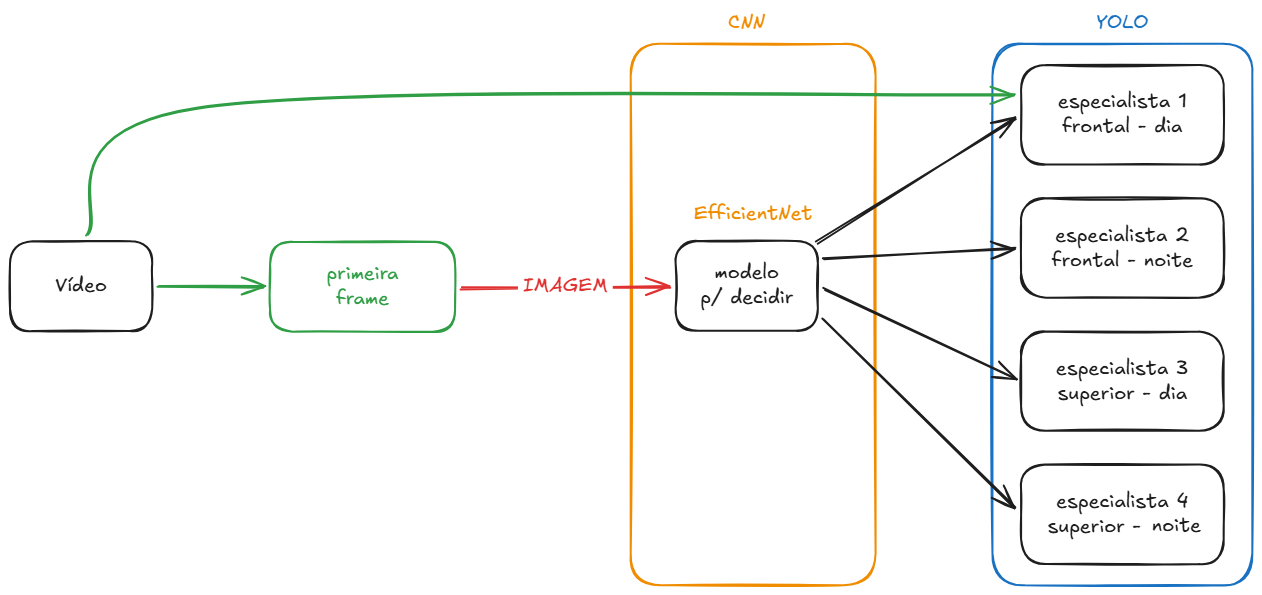
\includegraphics[width=\textwidth]{figs/moe.png}
\caption{Arquitetura MoE proposta: o primeiro quadro do vídeo é classificado pela rede de roteamento (EfficientNet-B0), que seleciona um dos quatro especialistas YOLOv8m; o especialista selecionado processa todos os quadros do vídeo.}
\label{fig:arquitetura-moe}

Fonte: Elaborada pelo autor.
\end{figure}

O \textit{pipeline} recebe um vídeo e executa os seguintes passos:
\begin{enumerate}
    \item O primeiro quadro do vídeo é lido e convertido para o espaço de cores RGB;
    \item O quadro passa pelo mesmo pré-processamento da validação da rede de roteamento (redimensionamento, recorte central em 224$\times$224 pixels e normalização do ImageNet) e é classificado pela EfficientNet-B0. As saídas da rede passam por uma função \textit{softmax}, e o cenário de maior probabilidade é escolhido; essa probabilidade é registrada como a confiança do roteamento;
    \item Os pesos do especialista correspondente ao cenário escolhido são carregados;
    \item O especialista processa todos os quadros do vídeo, com limiar de confiança de 0,7 e limiar de IoU de 0,7 para a supressão de não máximos (\textit{non-maximum suppression}, NMS), que elimina caixas sobrepostas atribuídas a um mesmo objeto;
    \item O vídeo anotado com as caixas detectadas e um relatório com o cenário identificado, a confiança do roteamento, o especialista usado e o tempo de processamento são salvos.
\end{enumerate}

O roteamento é feito uma única vez por vídeo, no primeiro quadro. Essa escolha parte do fato de que as câmeras são fixas: a perspectiva de um vídeo nunca muda, e a iluminação de uma sessão curta normalmente também não. Com isso, a rede de roteamento é executada uma vez, e o custo por quadro é o de um único YOLOv8m, igual ao do baseline. Em contrapartida, um erro de roteamento no primeiro quadro compromete o vídeo inteiro, e uma sessão que atravessasse o amanhecer ou o anoitecer continuaria a ser processada pelo especialista escolhido no início. O roteamento quadro a quadro, ou em intervalos regulares, eliminaria essa limitação ao custo de executar a rede de roteamento mais vezes.

\section{Avaliação em Vídeos de Teste}
\label{sec:avaliacao-videos}

\subsection{Vídeos de Teste e Verificação de Vazamento}
\label{subsec:videos-teste}

Além da validação cruzada, as duas abordagens foram avaliadas em quatro vídeos de teste, um por cenário, com 80 quadros cada (10 segundos a 8 FPS). Esses vídeos foram gravados na mesma baia. Os vídeos Frontal Dia e Frontal Noite vêm da câmera Cam03, e os vídeos Superior Dia e Superior Noite, da câmera Cam04.

Como os arquivos de teste não traziam metadados de data e hora nem seguiam o padrão de nome das sessões, foi preciso confirmar que nenhum deles era um recorte de uma sessão de treino. A verificação teve duas etapas. Na primeira, a data indicada no nome de cada vídeo foi comparada com as datas das sessões de treino. Essa comparação serve apenas como indício, pois várias sessões de câmeras diferentes podem ter a mesma data. Na segunda etapa, que é a decisiva, foram amostrados 12 quadros de cada vídeo de teste e comparados com as imagens de treino das sessões candidatas (as de mesma data ou, se nenhuma data coincidisse, todas as sessões). A comparação usou primeiro um \textit{hash} médio (\textit{average hash}) de 8$\times$8 bits, que descarta rapidamente pares muito diferentes: só seguiram para a etapa seguinte os pares com distância de Hamming de no máximo 12 bits. Os pares restantes foram comparados pelo erro quadrático médio (\textit{mean squared error}, MSE) entre os pixels das duas imagens, redimensionadas para 160$\times$160 pixels:
\begin{equation}
    \mathrm{MSE}(I, J) = \frac{1}{N} \sum_{k=1}^{N} \left( I_k - J_k \right)^2,
    \label{eq:mse}
\end{equation}
em que $I_k$ e $J_k$ são os valores do $k$-ésimo pixel e canal das duas imagens, e $N$ é o número total de valores.

O limiar de decisão foi calibrado na própria base. O MSE de uma imagem com ela mesma é zero, e o MSE entre dois quadros diferentes de uma mesma sessão de treino ficou entre cerca de 750 e 1.200, já que os animais se movem entre um quadro e outro. Um quadro de teste foi considerado duplicata de um quadro de treino apenas se o menor MSE encontrado fosse de no máximo 60, valor compatível com a diferença causada por uma nova compressão do mesmo quadro, e não com a de duas cenas parecidas. Como o pré-filtro por \textit{hash} pode descartar pares que, comparados pelo MSE, seriam próximos, a verificação foi repetida de forma exaustiva: todos os 80 quadros de cada vídeo de teste foram comparados, pelo MSE, com todas as imagens da base de detecção vindas da mesma câmera. Além disso, a câmera, a data e a hora gravadas na própria imagem pelo sistema de gravação foram lidas no primeiro quadro de cada vídeo de teste e comparadas com o intervalo de tempo coberto por cada sessão da base, obtido da mesma marcação no primeiro e no último quadro da sessão. Os resultados dessa verificação são apresentados no Capítulo~5.

\subsection{Protocolo de Inferência e Métrica de Contagem}
\label{subsec:metrica-contagem}

Os quatro vídeos foram processados pelo \textit{pipeline} MoE (Seção~\ref{sec:arquitetura-moe}) e pelo baseline monolítico, com o mesmo limiar de confiança (0,7), o mesmo limiar de IoU da supressão de não máximos (0,7) e a mesma resolução de entrada (640$\times$640 pixels).

Os vídeos de teste não têm rótulos, de modo que não é possível calcular precisão, revocação ou mAP sobre eles. A avaliação usou, em vez disso, a contagem de caixas. Como os oito animais estão sempre na baia, um detector sem erros produz exatamente oito caixas em cada quadro, ou $8 \times 80 = 640$ caixas por vídeo. Para cada abordagem e cada vídeo, foram registrados o total de caixas, o número de caixas por quadro e os quadros com menos ou mais de oito caixas. Menos de oito caixas indica animais não detectados; mais de oito indica detecções duplicadas ou falsos positivos.

A contagem total é uma medida grosseira, pois um animal perdido e uma caixa duplicada no mesmo quadro se compensam. Por isso, a análise também considerou a distribuição da contagem quadro a quadro e, nos quadros com mais de oito caixas, o IoU entre pares de caixas, para verificar se as caixas excedentes eram duplicatas sobre um mesmo animal que a supressão de não máximos deixou passar. Também foram registradas a confiança da rede de roteamento em cada vídeo e a faixa de confiança das caixas produzidas pelos especialistas. Os quadros com erros foram inspecionados visualmente, lado a lado, para as duas abordagens.

\section{Ambiente Computacional}
\label{sec:ambiente-computacional}

Os experimentos foram executados em um computador com sistema operacional Linux, processador de 16 núcleos e uma GPU NVIDIA GeForce RTX 5070 com 12 GB de memória. A base de imagens ficou armazenada em discos rígidos mecânicos. O código foi escrito em Python, em um ambiente Conda, com as bibliotecas PyTorch e \textit{torchvision} (rede de roteamento), Ultralytics (treinamento e inferência dos detectores YOLOv8), Captum (análise de oclusão), OpenCV (leitura de vídeos e extração de quadros), scikit-learn (divisão da base da rede de roteamento e métricas de classificação) e pandas, Matplotlib e seaborn (análise dos resultados e geração de gráficos).
